% OILTRACE — IEEE conference paper.
% Compile on Overleaf (pdfLaTeX) or locally with:  latexmk -pdf oiltrace.tex
% Every number below is traceable to a file in this repository; see paper/README.md.

\documentclass[conference]{IEEEtran}
\IEEEoverridecommandlockouts

\usepackage{cite}
\usepackage{amsmath,amssymb,amsfonts}
\usepackage{graphicx}
\usepackage{booktabs}
\usepackage{array}
\usepackage{textcomp}
\usepackage{xcolor}
\usepackage{url}
\usepackage{tikz}
\usetikzlibrary{arrows.meta,positioning,calc,shapes.geometric,fit}

\graphicspath{{figures/}}
\def\BibTeX{{\rm B\kern-.05em{\sc i\kern-.025em b}\kern-.08em
    T\kern-.1667em\lower.7ex\hbox{E}\kern-.125emX}}

% Figure styling shared by the three schematics.
\tikzset{
  box/.style={draw=black!70, rounded corners=2pt, fill=#1, align=center,
              font=\scriptsize, inner sep=3pt, minimum height=0.62cm},
  box/.default={black!4},
  flow/.style={-{Stealth[length=4pt]}, draw=black!70, line width=0.5pt},
  lbl/.style={font=\tiny, text=black!70, align=center},
}

\begin{document}

\title{OILTRACE: An Integrated Prototype for SAR Oil-Spill Tile Classification, AIS Anomaly Screening, Drift Estimation and Vessel Risk Planning}

% TODO before submission: replace the placeholders with the authors in the agreed
% order, and mark the corresponding author.
\author{\IEEEauthorblockN{[Author 1], [Author 2], [Author 3], [Author 4], [Author 5], [Author 6]}
\IEEEauthorblockA{Department of Computer Engineering and Technology\\
MIT World Peace University, Pune, India\\
Corresponding author: [name, e-mail]}}

\maketitle

\begin{abstract}
Investigating a marine oil spill requires more than finding a dark patch in a
satellite image. Investigators also need vessel movements, a plausible source
region, the likely drift of the oil and warnings for ships whose projected tracks
cross the affected area. OILTRACE is a software prototype that links these tasks.
It combines a convolutional neural network (CNN) that classifies synthetic aperture
radar (SAR) tiles, an Isolation Forest that screens Automatic Identification System
(AIS) tracks for unusual movement, rule-based source back-projection and vessel
ranking, a current-plus-windage drift envelope, risk-zone screening and geometric
detour candidates. On a scene-grouped held-out set of 574 tiles from 451 scenes of
a public Sentinel-1 dataset, the CNN reaches 96.34\% accuracy, 94.33\% precision,
94.82\% recall, 94.57\% F1-score and 0.9933 ROC-AUC. A perceptual-hash check shows
that removing the 58 test tiles with a near-duplicate in training leaves accuracy at
96.12\% and ROC-AUC at 0.9930. On 52,049 scoreable AIS rows from 347 vessels, an
anomaly-injection test on 69 vessels unseen during fitting gives 0.993 ROC-AUC and
86.2\% recall at a 0.9\% flag rate on unmodified rows. The end-to-end pipeline is
demonstrated on a constructed incident built from real, pseudonymised AIS tracks.
That scenario tests integration, not attribution accuracy.
\end{abstract}

\begin{IEEEkeywords}
Oil-spill detection, synthetic aperture radar, Sentinel-1, AIS anomaly detection,
Isolation Forest, maritime surveillance, drift estimation, decision support.
\end{IEEEkeywords}

% ---------------------------------------------------------------------------
\section{Introduction}

Oil spills arise from tanker accidents, equipment failure and illegal operational
discharge. Early detection shortens response time and helps focus containment
resources. SAR is well suited to the task because it images through cloud and at
night. Oil damps short surface waves and appears dark, but low-wind areas, biogenic
films and acquisition effects produce similar \emph{look-alikes}~\cite{brekke2005}.
Image-level detection on its own is therefore uncertain.

AIS broadcasts identity, position, speed over ground (SOG), course over ground (COG)
and time. Historical tracks let an investigator ask which vessels were near a
candidate release location and whether they moved unusually. AIS can be incomplete
or erroneous, however, and unusual movement does not establish intent. Drift estimates
and route suggestions add planning context, but they depend on environmental data and
navigation constraints.

Potdar~\emph{et~al.}~\cite{potdar2025} combined satellite imagery with AIS for spill
detection. OILTRACE builds on that idea and makes four contributions:
\begin{itemize}
  \item \textbf{Leakage-controlled image evaluation.} A tile classifier is evaluated
  on a split grouped by source scene, with exact-duplicate removal and a
  perceptual-hash near-duplicate audit. Its probabilities are calibrated by temperature
  scaling, and its decision threshold is fitted on validation data only.
  \item \textbf{Location-independent AIS screening.} AIS ``not available'' codes are
  handled explicitly, tracks are segmented at gaps, and an Isolation Forest is trained
  on movement features only. It is evaluated by anomaly injection on held-out vessels.
  \item \textbf{An assumption-explicit investigation chain.} The chain runs from source
  back-projection through a transparent three-factor vessel ranking to a counterfactual
  consistency test. A $7\times7$ drift-sensitivity sweep reports how much each verdict
  depends on the drift assumption.
  \item \textbf{Forward risk planning.} Projected vessel tracks are screened against
  buffered risk zones, and a geometric detour candidate is generated for each affected
  vessel. Results are presented in a web dashboard that labels each output by evidence
  type.
\end{itemize}

The guiding design rule is to keep model output separate from observation. The CNN
predicts a tile class, not a geographic boundary. A vessel score is an investigative
lead, not proof. A geometric route is not navigation advice.

% ---------------------------------------------------------------------------
\section{Related Work}

\subsection{Oil Detection in SAR Imagery}
Classical pipelines segment dark regions, extract shape and backscatter features,
and then classify each region as oil or look-alike~\cite{brekke2005}. Deep learning is
now widely used. Krestenitis~\emph{et~al.}~\cite{krestenitis2019} released a labelled
Sentinel-1 dataset and benchmarked semantic-segmentation networks.
Blondeau-Patissier~\emph{et~al.}~\cite{blondeau2023} combined deep learning with
empirical methods to detect oil-like features around the Great Barrier Reef, and
released the chip dataset~\cite{csiro2022} used here. Our CNN is simpler than a
segmentation network. It labels a whole tile and does not delineate the slick.

\subsection{AIS Movement Analysis}
Tu~\emph{et~al.}~\cite{tu2018} survey AIS cleaning and its uses, including anomaly
detection. Riveiro~\emph{et~al.}~\cite{riveiro2018} review maritime anomaly detection
more broadly. The Isolation Forest~\cite{liu2008} needs no labelled examples of
misconduct, because it relies on anomalous points being easier to isolate. This makes
it suitable when no ground truth exists.

\subsection{Oil Drift Modelling}
Operational tools such as OpenDrift~\cite{dagestad2018} advect many Lagrangian
particles under time-varying currents, wind and waves. A widely used first-order
approximation moves a slick with the vector sum of the surface current and a windage
term of a few percent, commonly about 3\%, of the wind velocity~\cite{asce1996,reed1999}.
We use this approximation with fixed inputs (Section~\ref{sec:drift}).

\subsection{Ship Route Planning}
Tam~\emph{et~al.}~\cite{tam2009} and Huang~\emph{et~al.}~\cite{huang2020} review route
planning and collision avoidance, from geometric constructions to graph search. Our
detour module uses a tangent--arc--tangent construction around a buffered zone. It makes
no claim of algorithmic novelty. Its role is to turn a risk polygon into a candidate
route within the pipeline.

% ---------------------------------------------------------------------------
\section{Data}

\subsection{SAR Image Chips}
\label{sec:sar}
The image data are the CSIRO Sentinel-1 SAR oil and non-oil chip
dataset~\cite{csiro2022}, released under CC BY-SA 4.0. It contains 5,630 grayscale
$400\times400$ JPEG chips: 3,725 in class~0 (no oil features, including look-alikes)
and 1,905 in class~1 (oil features). The label semantics are those documented by the
dataset authors. We obtained the files from a public mirror~\cite{mirror} and verified
that it is identical to the CSIRO release in file count and class counts. We use the
mirror rather than the renamed copy on Kaggle because only the original filenames carry
the source-scene identifier.

Each filename encodes a tile offset, a 16-character scene identifier and a region code.
Chips from one scene overlap by 50\%, and a few are rotated or cropped copies. We
removed 4 images whose byte-identical copy carries the opposite label and 90 exact
duplicates (MD5). This left 5,536 tiles in 4,492 scene groups (one filename that does
not parse forms its own group). Table~\ref{tab:sar} gives the split.

\begin{table}[t]
\caption{SAR Dataset and Scene-Grouped Split}
\label{tab:sar}
\centering
\footnotesize
\begin{tabular}{@{}lr@{}}
\toprule
Item & Value \\
\midrule
Source chips (class 0 / class 1) & 5,630 (3,725 / 1,905) \\
Removed: label conflicts / exact duplicates & 4 / 90 \\
Usable tiles / scene groups & 5,536 / 4,492 \\
Train: tiles (scenes) & 4,409 (3,597) \\
Validation: tiles (scenes) & 553 (444) \\
Test: tiles (scenes); oil share & 574 (451); 33.6\% \\
\bottomrule
\end{tabular}
\end{table}

\subsection{AIS Reference Corpus}
The AIS corpus is an extract in the MarineCadastre.gov export schema, published by
BOEM and NOAA from U.S.\ Coast Guard receivers~\cite{marinecadastre}. It covers the Gulf
of Mexico from 31~December 2020 to 28~March 2021 and contains 52,943 records from 347
vessels. It contains the AIS ``not available'' codes SOG\,=\,102.3~kn (132 rows),
COG\,=\,360\textdegree{} (446 rows) and heading\,=\,511 (2,938 rows). Cleaning recovers
all 132 missing SOG values and 251 of the COG values from consecutive positions, and
splits the tracks into 797 segments at gaps longer than 15~min. Feature construction
yields 52,049 scoreable rows.

\subsection{Integration Scenario}
\label{sec:scenario}
No public dataset pairs a SAR-observed spill with the AIS tracks of all nearby vessels,
so the end-to-end pipeline is exercised on a constructed scenario. Twelve vessels are
drawn from one traffic cluster in the corpus. Their recorded positions, speeds, courses
and dimensions are kept. Each vessel's timestamps are shifted by a constant offset onto
a shared clock of three passes four hours apart. The shift is needed because, measured
across the whole corpus, at most 3 of the 347 vessels carry a fix at all three passes.
The third pass receives oil-positive chips for two vessels by a seeded random draw, made
before any model runs. Because the scenario ranks vessels as suspects for a fictitious
incident, all twelve are shown under pseudonyms (Vessel~A--L).

\subsection{Environmental Inputs}
No measured current or wind field is used in this study. The drift computations use
stated values: surface current 0.25~m/s toward 170\textdegree, 10-m wind 5.0~m/s toward
200\textdegree{} and 3\% windage. The software accepts a gridded reanalysis (e.g.,
current and wind components on a regular latitude--longitude--time grid) and uses it
in place of these values when one is provided.

% ---------------------------------------------------------------------------
\section{System Architecture}

OILTRACE consists of a Python/FastAPI backend and a React/TypeScript dashboard with
Leaflet map overlays. PyTorch~\cite{paszke2019} runs the CNN, scikit-learn~\cite{pedregosa2011}
the Isolation Forest, and Shapely the geometric operations. Fig.~\ref{fig:workflow}
shows the workflow. Each response carries a provenance field that distinguishes live
inference, stored results and rule-based calculations.

\begin{figure}[t]
\centering
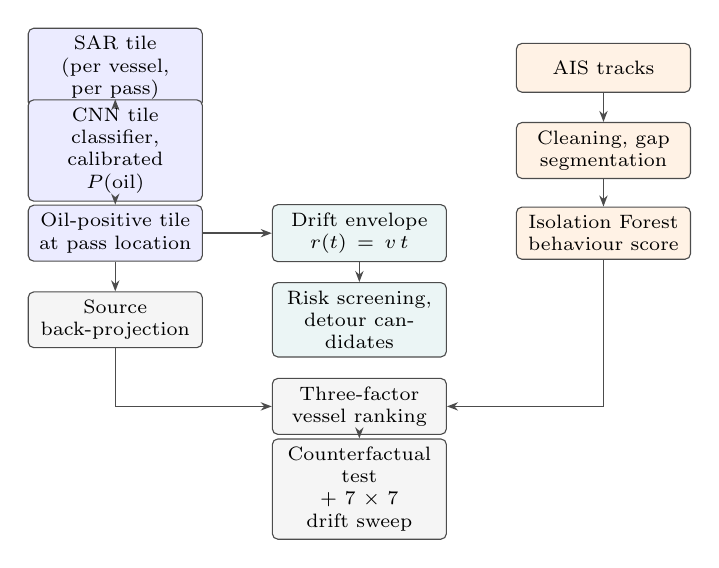
\begin{tikzpicture}[every node/.append style={minimum width=2.15cm, text width=2.0cm}]
  % Image branch (left), AIS branch (right), shared investigation chain (centre).
  \node[box={blue!8}]   (sar)   at (1.15, 0)    {SAR tile\\(per vessel, per pass)};
  \node[box={blue!8}]   (cnn)   at (1.15,-1.05) {CNN tile classifier,\\calibrated $P(\mathrm{oil})$};
  \node[box={blue!8}]   (det)   at (1.15,-2.1)  {Oil-positive tile\\at pass location};
  \node[box={orange!10}] (ais)  at (7.35, 0)    {AIS tracks};
  \node[box={orange!10}] (clean) at (7.35,-1.05) {Cleaning, gap\\segmentation};
  \node[box={orange!10}] (iso)  at (7.35,-2.1)  {Isolation Forest\\behaviour score};
  \node[box={teal!8}]   (env)   at (4.25,-2.1)  {Drift envelope\\$r(t)=v\,t$};
  \node[box={teal!8}]   (risk)  at (4.25,-3.2)  {Risk screening,\\detour candidates};
  \node[box]            (src)   at (1.15,-3.2)  {Source\\back-projection};
  \node[box]            (rank)  at (4.25,-4.3)  {Three-factor\\vessel ranking};
  \node[box]            (cf)    at (4.25,-5.35) {Counterfactual test\\+ $7\times7$ drift sweep};
  \draw[flow] (sar) -- (cnn);   \draw[flow] (cnn) -- (det);
  \draw[flow] (ais) -- (clean); \draw[flow] (clean) -- (iso);
  \draw[flow] (det) -- (env);   \draw[flow] (env) -- (risk);
  \draw[flow] (det) -- (src);
  \draw[flow] (src.south) |- (rank.west);
  \draw[flow] (iso.south) |- (rank.east);
  \draw[flow] (rank) -- (cf);
\end{tikzpicture}
\caption{OILTRACE workflow. The CNN marks a tile as oil-positive. The oil position is
the vessel's AIS fix at that pass, not a CNN localisation.}
\label{fig:workflow}
\end{figure}

\subsection{CNN Architecture}
Each tile is converted to grayscale, resized to $224\times224$, replicated to three
channels and normalised with mean 0.5 and standard deviation 0.5. There are four
convolutional blocks (32, 64, 128 and 256 channels). Each has two
convolution--batch-normalisation--ReLU stages followed by max pooling. Global average
pooling gives a 256-dimensional vector. The head is: dropout 0.30, a 256-to-128 linear
layer with ReLU, dropout, and a 128-to-2 linear layer. The network has 1,206,370
trainable parameters (Fig.~\ref{fig:cnn}).

\begin{figure}[t]
\centering
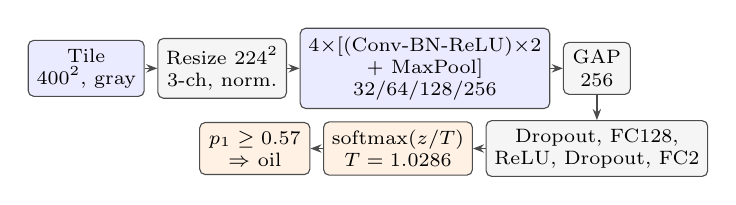
\begin{tikzpicture}[node distance=0.16cm]
  \node[box={blue!8}, minimum width=1.0cm] (in) {Tile\\$400^2$, gray};
  \node[box, right=of in, minimum width=1.05cm] (pre) {Resize $224^2$\\3-ch, norm.};
  \node[box={blue!8}, right=of pre, minimum width=1.6cm] (conv) {$4\times$[(Conv-BN-ReLU)$\times2$\\+ MaxPool]\\32/64/128/256};
  \node[box, right=of conv, minimum width=0.85cm] (gap) {GAP\\256};
  \node[box, below=0.32cm of gap, minimum width=1.5cm] (head) {Dropout, FC128,\\ReLU, Dropout, FC2};
  \node[box={orange!10}, left=of head, minimum width=1.6cm] (cal) {softmax$(z/T)$\\$T=1.0286$};
  \node[box={orange!10}, left=of cal, minimum width=1.4cm] (thr) {$p_1\ge0.57$\\$\Rightarrow$ oil};
  \draw[flow] (in) -- (pre); \draw[flow] (pre) -- (conv); \draw[flow] (conv) -- (gap);
  \draw[flow] (gap) -- (head); \draw[flow] (head) -- (cal); \draw[flow] (cal) -- (thr);
\end{tikzpicture}
\caption{CNN tile classifier and the validation-fitted output calibration.}
\label{fig:cnn}
\end{figure}

\subsection{AIS Anomaly Model}
The Isolation Forest uses 300 trees, contamination 0.02 and random seed 42, applied
after a StandardScaler. It has four inputs: SOG, acceleration (kn/min), turn rate
(\textdegree/min) and the mismatch between reported SOG and the speed implied by
consecutive positions. Latitude, longitude and raw course are excluded so that the
model learns motion, not a location or lane direction.

% ---------------------------------------------------------------------------
\section{Methods}

\subsection{CNN Calibration and Decision Rule}
Let $z_0,z_1$ be the no-oil and oil logits. With temperature $T$,
\begin{equation}
p_i=\frac{\exp(z_i/T)}{\sum_{j}\exp(z_j/T)},\qquad
\hat y=\begin{cases}1,& p_1\ge\tau\\0,&\text{otherwise.}\end{cases}
\end{equation}
Temperature scaling~\cite{guo2017} sets $T=1.0286$ by minimising validation
log-loss (L-BFGS). $\tau=0.57$ maximises validation F1
over a sweep from 0.05 to 0.95 in steps of 0.01. Neither value was fitted on the test set.

\subsection{Evaluation Measures and Uncertainty}
From the true/false positives and negatives (TP, TN, FP, FN):
\begin{gather}
\text{Accuracy}=\tfrac{TP+TN}{TP+TN+FP+FN},\quad
\text{Specificity}=\tfrac{TN}{TN+FP},\\
\text{Precision}=\tfrac{TP}{TP+FP},\quad
\text{Recall}=\tfrac{TP}{TP+FN},\quad
F_1=\tfrac{2\,\text{Prec}\cdot\text{Rec}}{\text{Prec}+\text{Rec}}.
\end{gather}
ROC-AUC and average precision are threshold-free and take oil as the positive class.
Expected calibration error (ECE) uses 10 equal-width probability bins. Tiles from one
scene are not independent, so 95\% confidence intervals come from a scene-cluster
bootstrap. Each of 1,000 resamples draws whole test scenes with replacement, and the
interval is the 2.5th--97.5th percentile.

\subsection{AIS Cleaning and Movement Features}
Records are sorted by vessel and time. Sentinel codes become missing values, and SOG
above 50~kn is treated as invalid. SOG and COG are recovered from consecutive positions
where possible. A gap over 15~min starts a new segment, and no feature spans a gap.
Great-circle distance uses the haversine formula ($R=6{,}371.0088$~km, angles in radians):
\begin{gather}
a=\sin^2\!\tfrac{\varphi_2-\varphi_1}{2}+\cos\varphi_1\cos\varphi_2\sin^2\!\tfrac{\Delta\lambda}{2},\\
d=2R\arcsin\sqrt{a},\qquad v_{\mathrm{impl}}=\frac{d}{1.852\,\Delta t}\ \text{[kn]},
\end{gather}
with $\Delta t$ in hours. Acceleration is $\Delta\mathrm{SOG}/\Delta t_{\min}$. The circular
course change is $\Delta\theta=\min(\delta,360^\circ-\delta)$ with
$\delta=|\theta_t-\theta_{t-1}|\bmod 360^\circ$, and turn rate is
$\Delta\theta/\Delta t_{\min}$. The speed mismatch is $m=|\mathrm{SOG}-v_{\mathrm{impl}}|$.
The raw anomaly score $s=-f(\mathbf{x})$ (the negated decision function) is mapped to a
0--100 score by linear interpolation between the training median (0) and the training
99.5th percentile (100). The result is clipped. Rows with a missing feature are not
scored.

\subsection{Source Estimate and Vessel Ranking}
A tile that is clear in one pass and oil-positive in the next bounds the release to the
interval between the passes (4~h in the scenario). The source is back-projected from the
oil-positive position by displacement $D=vt$ along compass bearing $\theta$, measured
clockwise from true north:
\begin{equation}
\Delta E=-D\sin\theta,\qquad \Delta N=-D\cos\theta.
\end{equation}
Vessels with an AIS fix within $\pm2$~h of the release time and within a search radius
$r$ of the source are ranked. The radius is three drift-envelope radii, $r=3\,v_{\mathrm{drift}}t$
(16.7~km at 4~h), so traffic that could not plausibly be the source is filtered out. The
ranking score is
\begin{equation}
S=0.40\,P+0.30\,G+0.30\,B,\quad P=\mathrm{clip}\!\left[100\left(1-\tfrac{d_{\min}}{r}\right),0,100\right],
\label{eq:rank}
\end{equation}
where $d_{\min}$ is the closest approach to the source in the release window. The
trajectory-convergence term is $G=\mathrm{clip}[100(d_0-d'_{\min})/d_0,0,100]$. Here $d_0$
and $d'_{\min}$ are the first and the smallest distance to the source over a window from
6~h before to 2~h after release. $B$ is the vessel's maximum calibrated anomaly score over
its track. If $B$ is unavailable, $P$ and $G$ are renormalised to sum to one rather than setting $B$
to zero. A separate seven-factor attribution score in the AIS module is not used by the
dashboard (Table~\ref{tab:scores}). Both are hand-weighted heuristics. They give
investigation priority, not a probability of culpability.

\begin{table}[t]
\caption{Scoring Rules in the Codebase}
\label{tab:scores}
\centering
\footnotesize
\begin{tabular}{@{}p{1.6cm}p{4.0cm}p{1.6cm}@{}}
\toprule
Score & Components (weight) & Used by \\
\midrule
Vessel ranking & proximity (0.40), trajectory (0.30), behaviour (0.30) & Dashboard, Eq.~\eqref{eq:rank} \\
Attribution prototype & release-time match (20), source overlap (25), trajectory (20), distance (15), behaviour (10), AIS consistency (5), vessel relevance (5) & AIS module only \\
Response priority & envelope area (0.45), confidence (0.30), vessel length (0.25) & Dashboard, Eq.~\eqref{eq:priority} \\
\bottomrule
\end{tabular}
\end{table}

\subsection{Drift Paths}
\label{sec:drift}
The system carries three constant drift vectors (Table~\ref{tab:drift}). The
environment-aware vector is the sum of current and windage, with all bearings in
degrees clockwise from north and speeds converted to km/h:
\begin{gather}
E=v_c\sin\theta_c+0.03\,v_w\sin\theta_w,\quad
N=v_c\cos\theta_c+0.03\,v_w\cos\theta_w,\\
v_{\mathrm{drift}}=\sqrt{E^2+N^2},\qquad
\theta_{\mathrm{drift}}=\operatorname{atan2}(E,N)\bmod 360^\circ.
\end{gather}
The stated inputs give 0.90~km/h of current and 0.54~km/h of windage, so
$v_{\mathrm{drift}}\approx1.394$~km/h toward $181.2^\circ$. The other two vectors are fixed
scenario constants inherited from our earlier prototype. We kept them, rather than
replacing them, so that the dashboard can show the result under both a fixed
kinematic assumption and an environment-derived one, and report where the two
disagree. The disagreement measures sensitivity to an assumption. It is not a
forecast error. Each vector is used consistently within its own path. The
counterfactual consistency radius, for example, is computed from the same vector that
moves the oil.

\begin{table}[t]
\caption{Drift Vectors and Where Each Is Used}
\label{tab:drift}
\centering
\footnotesize
\begin{tabular}{@{}p{2.15cm}p{1.75cm}p{3.4cm}@{}}
\toprule
Path & Vector & Used for \\
\midrule
Kinematic hindcast & 1.5 km/h $\to$ 135\textdegree & Source estimate, ranking, legacy counterfactual \\
Kinematic forecast & 1.0 km/h $\to$ 180\textdegree & Positions at $+6$, $+12$, $+24$, $+48$~h \\
Environment-aware & 1.394 km/h $\to$ 181.2\textdegree & Drift envelope, environment-aware source, ranking and counterfactual \\
\bottomrule
\end{tabular}
\end{table}

The drift envelope is a circle of radius $r(t)=v_{\mathrm{drift}}\,t$ and area
$A(t)=\pi r(t)^2$. It is the region the oil could have reached, not a measured slick
area.

\subsection{Counterfactual Test and Sensitivity Sweep}
For a candidate vessel, the counterfactual test moves a parcel from the vessel's AIS
position at the estimated release time forward along the drift vector for the
estimated age. It reports the miss distance to the observed oil position. The verdict
is \emph{consistent} if the miss is within the distance that drift can carry oil in that
time. To show how much the verdict depends on the assumed vector, it is re-evaluated on
a $7\times7$ grid. The grid spans speed $\pm50\%$ (0.75--2.25~km/h about the hindcast)
and bearing $\pm45^\circ$ (90--180\textdegree), which contains all three vectors in
Table~\ref{tab:drift}. A verdict is \emph{robust} if at least 90\% of the 49 evaluations
agree and \emph{moderately sensitive} at 60--90\%. The sweep is deterministic and is not a
probability distribution.

\subsection{Risk Screening and Detour Candidates}
Each vessel's track is projected 6~h ahead and intersected with the current and forecast
risk polygons, buffered by 3~km. The reroute service merges and buffers the polygons,
builds four tangent--arc--tangent candidates around an enclosing circle, discards any that
intersect the risk geometry and returns the shortest valid one (Fig.~\ref{fig:detour}).
A vessel already inside a zone receives an exit route, labelled as such. Shipping lanes,
bathymetry, traffic, manoeuvring limits and COLREGs are not modelled.

\begin{figure}[t]
\centering
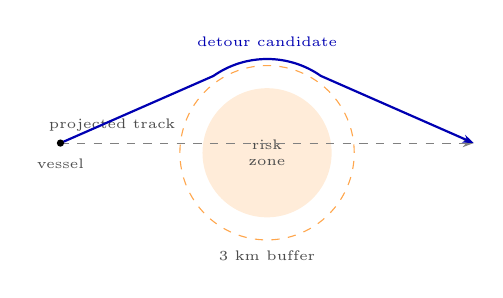
\begin{tikzpicture}[scale=0.82]
  \fill[orange!15] (0,0) circle (1.0);
  \draw[orange!70, dashed] (0,0) circle (1.35);
  \node[lbl] at (0,0) {risk\\zone};
  \node[lbl] at (0.0,-1.6) {3 km buffer};
  \draw[black!50, dashed, -{Stealth[length=4pt]}] (-3.2,0.15) -- (3.2,0.15);
  \node[lbl, anchor=south] at (-2.4,0.18) {projected track};
  \draw[blue!70!black, thick, -{Stealth[length=4pt]}]
     (-3.2,0.15) -- (-0.83,1.19) arc (125:55:1.45) -- (3.2,0.15);
  \node[lbl, text=blue!70!black] at (0,1.72) {detour candidate};
  \fill (-3.2,0.15) circle (1.6pt);
  \node[lbl, anchor=north] at (-3.2,0.05) {vessel};
\end{tikzpicture}
\caption{Schematic of the tangent--arc--tangent detour around a buffered zone (not to
scale). It is an illustration, not a benchmark route.}
\label{fig:detour}
\end{figure}

\subsection{Response Priority}
When several detections are present, a relative triage score orders them:
\begin{equation}
Q=0.45A_n+0.30C_n+0.25L_n,
\label{eq:priority}
\end{equation}
with $A_n=\mathrm{clip}(100A/400,0,100)$ for envelope area $A$ in km$^2$,
$L_n=\mathrm{clip}(100L/330,0,100)$ for the length $L$ in metres of the vessel at the
detection position, and $C_n$ the calibrated CNN probability in percent. The weights and
caps are configured, not fitted. $Q$ excludes oil volume, thickness, shoreline distance,
habitat sensitivity and weathering, so it is not a damage estimate.

% ---------------------------------------------------------------------------
\section{Experimental Setup}

\subsection{CNN Training}
Splitting uses \texttt{StratifiedGroupKFold} (10 folds, shuffled, seed 42) grouped by
scene. Fold~0 is the test set, fold~1 the validation set and the rest the training set.
Assertions confirm that no scene appears in two partitions. Training uses AdamW~\cite{loshchilov2019}
(learning rate $10^{-3}$, weight decay $10^{-4}$), cross-entropy loss, batch size 32,
gradient clipping at 2.0 and a ReduceLROnPlateau schedule on validation ROC-AUC
(factor 0.5, patience 3). Augmentation is applied to training data only. The checkpoint
with the best validation ROC-AUC is kept. Early stopping uses a patience of 8 epochs
within a 50-epoch cap. It did not trigger: validation ROC-AUC was still improving
slowly and peaked at 0.9903 in epoch~50, varying only between 0.986 and 0.990 over
epochs 43--50 (Fig.~\ref{fig:training}). The run is therefore cap-limited. A longer run
might add a small gain, which we did not pursue so that the evaluated model stays fixed.

\subsection{Near-Duplicate Audit}
Grouping by filename scene ID cannot catch the same sea patch filed under a different
ID, or a rotated copy. We computed a 64-bit DCT perceptual hash for every tile. Each
validation and test tile was hashed in all eight orientations (four rotations, with and
without mirroring). A tile counts as a near-duplicate if its Hamming distance to any
training tile is at most 8 bits (strict: 4 bits). The fixed model was then re-scored on
the test tiles that have no such match.

\subsection{AIS Evaluation}
No labelled misconduct exists in the corpus, so the AIS model is evaluated by injection.
Vessels, not rows, are split: 69 of 347 vessels (20\%) are held out. A separate
evaluation model, including its scaler and score calibration, is fitted only on the
remaining 278 vessels. In the 7,977 scoreable held-out rows, 160 rows (2\%) are modified
with one of three patterns, each with a fixed seed: \emph{speed collapse} (acceleration
1.5--4.0~kn/min), \emph{erratic turns} (40--120\textdegree/min) and \emph{position jump}
(speed mismatch 6--15~kn). The model used by the dashboard is a different fit, trained on
all 52,049 rows.

% ---------------------------------------------------------------------------
\section{Results}

\subsection{CNN on the Held-Out Test Set}
Table~\ref{tab:cnn} and Figs.~\ref{fig:confusion}--\ref{fig:roc} report the test results.
The classifier labels 553 of 574 tiles correctly. Of 193 oil tiles it finds 183, and 11 of
its 194 oil predictions are false positives. The scene-bootstrap 95\% intervals are
94.59--97.91\% for accuracy, 90.51--97.42\% for precision, 90.66--98.07\% for recall and
0.9869--0.9977 for ROC-AUC. Calibration is good both before and after temperature scaling.
Because $T$ is close to one, scaling changes little: validation ECE is 0.0229 before and
0.0238 after, and test ECE is 0.0140 (Fig.~\ref{fig:reliability}). Grad-CAM~\cite{selvaraju2017}
maps highlight the dark linear features on oil tiles (Fig.~\ref{fig:gradcam}). These maps
are a visual aid, not a segmentation.

\begin{table}[t]
\caption{CNN Held-Out Test Metrics (574 Tiles, 451 Scenes)}
\label{tab:cnn}
\centering
\footnotesize
\begin{tabular}{@{}lrr@{}}
\toprule
Metric & All tiles & No train near-dup.\ ($n{=}516$) \\
\midrule
Accuracy & 96.34\% & 96.12\% \\
Precision & 94.33\% & 94.19\% \\
Recall & 94.82\% & 94.19\% \\
F1-score & 94.57\% & 94.19\% \\
Specificity & 97.11\% & 97.09\% \\
ROC-AUC & 0.9933 & 0.9930 \\
Average precision & 0.9888 & --- \\
ECE (10 bins) & 0.0140 & --- \\
\bottomrule
\end{tabular}
\end{table}

\begin{figure}[t]
\centering
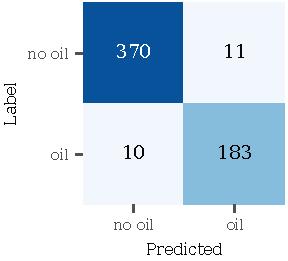
\includegraphics[width=0.52\columnwidth]{fig_confusion.pdf}
\caption{Confusion matrix on the held-out test set (TN 370, FP 11, FN 10, TP 183).}
\label{fig:confusion}
\end{figure}

\begin{figure}[t]
\centering
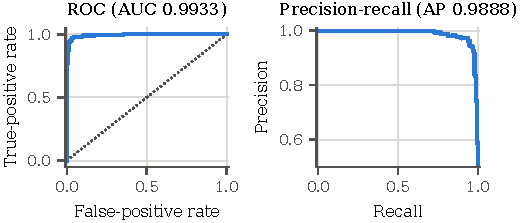
\includegraphics[width=\columnwidth]{fig_roc_pr.pdf}
\caption{ROC and precision--recall curves on the held-out test set.}
\label{fig:roc}
\end{figure}

\begin{figure}[t]
\centering
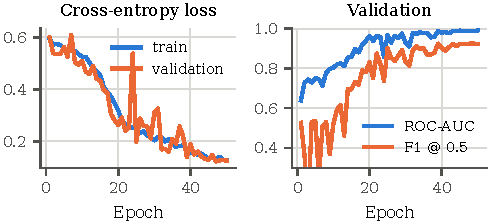
\includegraphics[width=\columnwidth]{fig_training.pdf}
\caption{Training curves. Validation F1 is shown at a fixed 0.5 threshold. The deployed
threshold (0.57) was chosen after training.}
\label{fig:training}
\end{figure}

\begin{figure}[t]
\centering
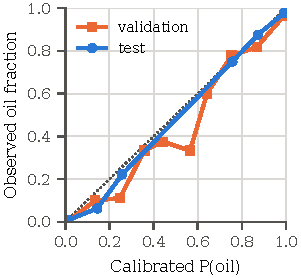
\includegraphics[width=0.55\columnwidth]{fig_reliability.pdf}
\caption{Reliability diagram after temperature scaling (10 bins, bins with fewer than 5
tiles omitted). The dotted line is perfect calibration.}
\label{fig:reliability}
\end{figure}

\begin{figure}[t]
\centering
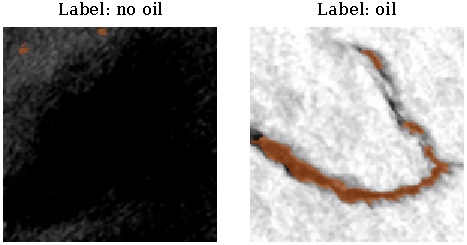
\includegraphics[width=\columnwidth]{fig_gradcam.pdf}
\caption{Grad-CAM regions refined by darkness on a no-oil and an oil chip. Chips from the
CSIRO dataset~\cite{csiro2022} (CC BY-SA 4.0), containing modified Copernicus Sentinel-1 data.}
\label{fig:gradcam}
\end{figure}

\subsection{Near-Duplicate Audit Results}
At the 8-bit threshold, 58 of 574 test tiles (52 scenes) and 52 of 553 validation tiles
have a near-duplicate in training. At the strict 4-bit threshold the counts are 7 and 9.
Removing all 58 test tiles changes accuracy from 96.34\% to 96.12\% and ROC-AUC from 0.9933
to 0.9930 (Table~\ref{tab:cnn}). The 8-bit threshold is deliberately loose, and smooth
open-sea chips can share a hash without sharing content. Even so, near-duplicate leakage
does not explain the test performance.

\subsection{AIS Anomaly Screening Results}
Table~\ref{tab:ais} summarises the results. The deployed model flags 1,041 of 52,049 rows
(2.00\%), which matches its contamination setting by construction. In the held-out
injection test, the anomaly score separates injected from unmodified rows with ROC-AUC
0.993. At the model's own flag threshold, it detects 86.2\% of injected rows and flags 0.9\%
of unmodified rows. By pattern, it flags 78.8\% of speed collapses, 80.4\% of erratic turns
and 98.2\% of position jumps. These figures show sensitivity to the injected patterns. They
do not show sensitivity to real discharges, which may not resemble them.

\begin{table}[t]
\caption{AIS Anomaly Evaluation}
\label{tab:ais}
\centering
\footnotesize
\begin{tabular}{@{}lr@{}}
\toprule
Measure & Value \\
\midrule
Raw records / vessels / segments & 52,943 / 347 / 797 \\
Scoreable rows; flagged by deployed model & 52,049; 1,041 (2.00\%) \\
\midrule
\multicolumn{2}{@{}l}{\emph{Injection test (model fitted on 278 other vessels)}} \\
Held-out vessels / rows / injected rows & 69 / 7,977 / 160 \\
ROC-AUC (injected vs.\ unmodified) & 0.993 \\
Recall on injected rows & 86.2\% \\
Flag rate on unmodified rows & 0.9\% \\
\bottomrule
\end{tabular}
\end{table}

\subsection{Integration Scenario Outcomes}
In the third pass, the CNN marks the chips of Vessels~B and~A as oil-positive. For the
first detection, the 4-h envelope has $r=1.394\times4\approx5.58$~km and
$A=\pi r^2\approx97.7$~km$^2$. The 16.7-km search radius admits 11 of the 12 vessels for
this detection and 5 of 12 for the second. Fig.~\ref{fig:scenario} shows the geometry
and Table~\ref{tab:cf} the leading candidates. Under the kinematic hindcast, Vessel~K
ranks first. Under the environment-aware drift, whose source estimate lies 4.56~km away,
Vessel~L moves from fourth to first and Vessel~K drops to second. The dashboard reports
this disagreement and labels the outcome ``leading candidate unstable''. Only Vessel~H's
verdict survives the whole sweep. For the second detection, none of the five candidates
is consistent under either drift, and the dashboard reports that no candidate is
supported. These outcomes show that the chain runs end to end and makes its dependence
on assumptions visible. They are not attribution accuracy, because the incident is
constructed. Fig.~\ref{fig:dashboard} shows the dashboard.

\begin{table}[t]
\caption{Scenario Detection 1: Top-Five Candidates}
\label{tab:cf}
\centering
\footnotesize
\begin{tabular}{@{}lrrll@{}}
\toprule
Vessel & $S$ & Miss (km) & Verdict & Sweep \\
\midrule
K & 86.44 & 2.88 & consistent & moderately sensitive \\
B & 73.45 & 4.37 & consistent & moderately sensitive \\
H & 72.71 & 9.15 & not consistent & robust \\
L & 68.79 & 3.82 & consistent & moderately sensitive \\
C & 66.85 & 8.41 & not consistent & moderately sensitive \\
\bottomrule
\multicolumn{5}{@{}p{0.95\columnwidth}@{}}{\scriptsize Kinematic counterfactual; the
consistency radius is $1.5\times4=6.00$~km.}
\end{tabular}
\end{table}

\begin{figure}[t]
\centering
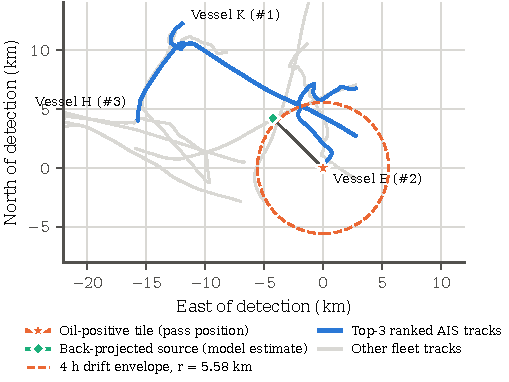
\includegraphics[width=\columnwidth]{fig_scenario.pdf}
\caption{Constructed scenario, first detection: pseudonymised AIS tracks, the
back-projected source and the 4-h drift envelope.}
\label{fig:scenario}
\end{figure}

\begin{figure}[t]
\centering
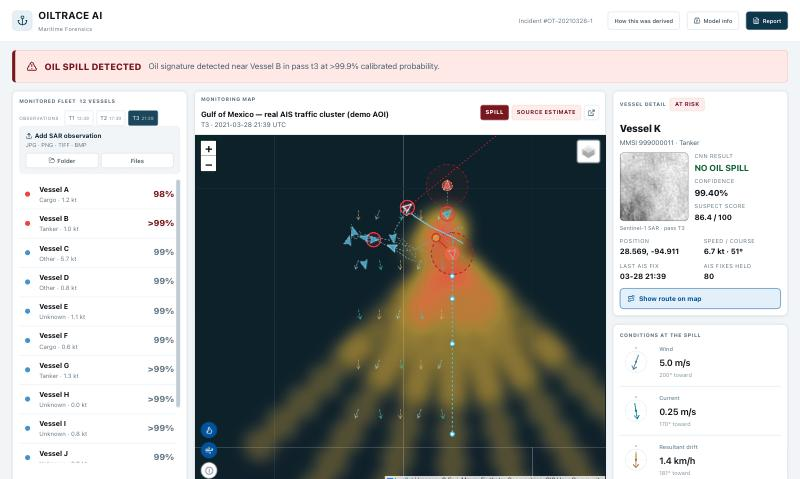
\includegraphics[width=\columnwidth]{fig_dashboard.jpg}
\caption{OILTRACE dashboard on the constructed scenario (pseudonymised vessels). Basemap
\textcopyright~Esri, Maxar, Earthstar Geographics. SAR chips from~\cite{csiro2022}.}
\label{fig:dashboard}
\end{figure}

% ---------------------------------------------------------------------------
\section{Discussion}

\subsection{Levels of Evidence}
The results fall into four kinds of evidence, which answer different questions. The CNN
metrics are \emph{measured} on a held-out partition of one public dataset. The AIS
injection metrics are measured in a \emph{controlled} experiment with artificial patterns.
The source estimate, envelope, forecast points, rankings and priority score are
\emph{rule-based calculations} on stated inputs. The scenario is \emph{constructed}. In
particular, a high CNN ROC-AUC does not establish localisation, and a high injection
ROC-AUC does not establish detection of real misconduct. A route that avoids a buffered
polygon is not thereby safe at sea.

\subsection{Comparison with Our Earlier Prototype}
Our earlier prototype reported 89.91\% accuracy and 71.35\% recall for a 421,570-parameter
CNN on a random tile-level split of 555 tiles. The present model reaches 96.34\% and 94.82\%
on a scene-grouped split. The two results are not comparable. Overlapping crops leak across
a random split, and the models, preprocessing and thresholds also differ. A fair comparison
would retrain both models on the same grouped split. The present version adds calibration,
explicit handling of AIS not-available codes, track segmentation, the environment-aware drift
path, the counterfactual sweep, forward risk screening and detour candidates.

\subsection{Interpretation of Scores}
A vessel's behaviour term is the maximum anomaly score over its track. A single unusual
record can therefore raise it, so the score should be read alongside the track and its
data quality. The four AIS features omit absolute position. This reduces dependence on
geography but does not remove distribution shift: vessel mix, reporting rate and normal
speeds differ between regions.

% ---------------------------------------------------------------------------
\section{Limitations}

\emph{Image model.} The CNN is evaluated on one dataset and one scene-grouped partition.
Its behaviour on other sensors, polarisations, regions and sea states is unknown. It
outputs a tile label, not a slick boundary, thickness or volume. Any spill coordinate
comes from the vessel's pass position, not from the CNN.

\emph{AIS model.} There is no ground truth of confirmed illegal discharges. Legitimate
manoeuvres, GPS errors and data corruption can raise scores, and a low score does not
establish normal behaviour. The ranking weights are set by hand and have not been
validated on confirmed sources.

\emph{Drift and routing.} No measured current or wind field and no observed slick
trajectory are used. The three constant vectors are assumptions, and the envelope is a
circle. Detours ignore traffic, bathymetry and COLREGs and are not navigation advice.

\emph{Scenario.} The incident uses time-shifted real tracks and seeded image assignments.
It demonstrates integration, not end-to-end accuracy on a real spill.

% ---------------------------------------------------------------------------
\section{Future Work: An Indian Deployment Path}

The models were developed on public Gulf of Mexico AIS and globally sourced Sentinel-1
chips. Several steps would make OILTRACE relevant to Indian waters:
\begin{enumerate}
  \item fine-tuning and re-evaluating the CNN on Sentinel-1 scenes over the Arabian Sea and
  Bay of Bengal with expert-verified labels, and reporting per-region performance;
  \item replacing the stated environmental inputs with INCOIS ocean-current products and IMD
  wind fields through the existing grid interface, and validating drift against observed
  slick trajectories from documented incidents;
  \item re-fitting the AIS model on Indian coastal AIS and assembling expert-labelled
  anomaly cases with the Indian Coast Guard;
  \item evaluating route candidates against charted traffic-separation schemes and
  bathymetry before any operational use.
\end{enumerate}

% ---------------------------------------------------------------------------
\section{Conclusion}

OILTRACE links SAR tile classification, AIS behaviour screening, source back-projection,
vessel ranking, a counterfactual drift sweep, risk screening and detour candidates in one
assumption-explicit pipeline. The strongest quantitative evidence is the CNN: 96.34\%
accuracy and 0.9933 ROC-AUC on 574 held-out tiles from 451 unseen scenes. This result is
essentially unchanged once tiles with a training near-duplicate are removed. The AIS
model separates injected anomalies from normal traffic on unseen vessels with 0.993
ROC-AUC. The constructed scenario shows that the chain runs end to end and reports when
its answer depends on an unmeasured drift assumption. Moving from prototype to operational
tool requires independent SAR scenes with verified labels, expert-labelled AIS cases,
measured environmental forcing, observed slick trajectories and route evaluation under
real maritime constraints.

\section*{Data and Code Availability}
Source code, trained model weights, the split manifest, per-tile test predictions and the
scripts that reproduce every table and figure are available at [repository URL]. The SAR
chips are available from CSIRO~\cite{csiro2022} under CC BY-SA 4.0, and the AIS data from
MarineCadastre.gov~\cite{marinecadastre}.

\section*{Acknowledgment}
The authors thank Dr.~Pramod Mali for his guidance throughout this project, and for his
feedback on experimental design, the interpretation of results and academic writing. We
also thank the Department of Computer Engineering and Technology, MIT World Peace
University, Pune, for its academic support and resources.

% Every entry was checked against its publisher or DOI record (see paper/README.md).
\begin{thebibliography}{00}
\bibitem{brekke2005} C.~Brekke and A.~H.~S. Solberg, ``Oil spill detection by satellite
remote sensing,'' \emph{Remote Sens. Environ.}, vol.~95, no.~1, pp.~1--13, 2005,
doi: 10.1016/j.rse.2004.11.015.

\bibitem{potdar2025} G.~P. Potdar, O.~L. Shinde, A.~S. Wadgaonkar, and A.~A. Mhetre,
``Detecting oil spills at marine environment using Automatic Identification System (AIS)
and satellite datasets,'' \emph{J. Eng. Technol. Manage.}, vol.~75, 2025. [Online].
Available: \url{https://jet-m.com/wp-content/uploads/48-JETM8851.pdf}

\bibitem{krestenitis2019} M.~Krestenitis, G.~Orfanidis, K.~Ioannidis, K.~Avgerinakis,
S.~Vrochidis, and I.~Kompatsiaris, ``Oil spill identification from satellite images using
deep neural networks,'' \emph{Remote Sens.}, vol.~11, no.~15, Art.~no.~1762, 2019,
doi: 10.3390/rs11151762.

\bibitem{blondeau2023} D.~Blondeau-Patissier, T.~Schroeder, G.~Suresh, Z.~Li,
F.~I. Diakogiannis, P.~Irving, C.~Witte, and A.~D.~L. Steven, ``Detection of marine
oil-like features in Sentinel-1 SAR images by supplementary use of deep learning and
empirical methods: Performance assessment for the Great Barrier Reef marine park,''
\emph{Mar. Pollut. Bull.}, vol.~188, Art.~no.~114598, 2023,
doi: 10.1016/j.marpolbul.2023.114598.

\bibitem{csiro2022} D.~Blondeau-Patissier, T.~Schroeder, F.~Diakogiannis, and Z.~Li,
``CSIRO Sentinel-1 SAR image dataset of oil- and non-oil features for machine learning
(Deep Learning),'' CSIRO Data Collection, v1, 2022, doi: 10.25919/4v55-dn16.

\bibitem{tu2018} E.~Tu, G.~Zhang, L.~Rachmawati, E.~Rajabally, and G.-B. Huang,
``Exploiting AIS data for intelligent maritime navigation: A comprehensive survey from
data to methodology,'' \emph{IEEE Trans. Intell. Transp. Syst.}, vol.~19, no.~5,
pp.~1559--1582, 2018, doi: 10.1109/TITS.2017.2724551.

\bibitem{riveiro2018} M.~Riveiro, G.~Pallotta, and M.~Vespe, ``Maritime anomaly
detection: A review,'' \emph{WIREs Data Mining Knowl. Discov.}, vol.~8, no.~5,
Art.~no.~e1266, 2018, doi: 10.1002/widm.1266.

\bibitem{liu2008} F.~T. Liu, K.~M. Ting, and Z.-H. Zhou, ``Isolation forest,'' in
\emph{Proc. 8th IEEE Int. Conf. Data Mining (ICDM)}, 2008, pp.~413--422,
doi: 10.1109/ICDM.2008.17.

\bibitem{dagestad2018} K.-F. Dagestad, J.~R\"ohrs, \O.~Breivik, and B.~{\AA}dlandsvik,
``OpenDrift v1.0: A generic framework for trajectory modelling,'' \emph{Geosci. Model
Dev.}, vol.~11, pp.~1405--1420, 2018, doi: 10.5194/gmd-11-1405-2018.

\bibitem{asce1996} ASCE Task Committee on Modeling of Oil Spills, ``State-of-the-art
review of modeling transport and fate of oil spills,'' \emph{J. Hydraul. Eng.}, vol.~122,
no.~11, pp.~594--609, 1996, doi: 10.1061/(ASCE)0733-9429(1996)122:11(594).

\bibitem{reed1999} M.~Reed, \O.~Johansen, P.~J. Brandvik, P.~Daling, A.~Lewis, R.~Fiocco,
D.~Mackay, and R.~Prentki, ``Oil spill modeling towards the close of the 20th century:
Overview of the state of the art,'' \emph{Spill Sci. Technol. Bull.}, vol.~5, no.~1,
pp.~3--16, 1999.

\bibitem{tam2009} C.~Tam, R.~Bucknall, and A.~Greig, ``Review of collision avoidance and
path planning methods for ships in close range encounters,'' \emph{J. Navig.}, vol.~62,
no.~3, pp.~455--476, 2009, doi: 10.1017/S0373463308005134.

\bibitem{huang2020} Y.~Huang, L.~Chen, P.~Chen, R.~R. Negenborn, and P.~H.~A.~J.~M. van
Gelder, ``Ship collision avoidance methods: State-of-the-art,'' \emph{Saf. Sci.},
vol.~121, pp.~451--473, 2020, doi: 10.1016/j.ssci.2019.09.018.

\bibitem{mirror} Saisamarth21, ``Oil-Spill-Detection-in-Marine-Environments-Using-AIS-and-Satellite-Data,''
GitHub repository (mirror of~\cite{csiro2022}). [Online]. Available:
\url{https://github.com/Saisamarth21/Oil-Spill-Detection-in-Marine-Environments-Using-AIS-and-Satellite-Data}

\bibitem{marinecadastre} Bureau of Ocean Energy Management and National Oceanic and
Atmospheric Administration, ``MarineCadastre.gov: AIS vessel traffic data,'' 2021.
[Online]. Available: \url{https://hub.marinecadastre.gov}

\bibitem{paszke2019} A.~Paszke \emph{et~al.}, ``PyTorch: An imperative style,
high-performance deep learning library,'' in \emph{Adv. Neural Inf. Process. Syst.},
vol.~32, 2019, pp.~8024--8035.

\bibitem{pedregosa2011} F.~Pedregosa \emph{et~al.}, ``Scikit-learn: Machine learning in
Python,'' \emph{J. Mach. Learn. Res.}, vol.~12, pp.~2825--2830, 2011.

\bibitem{guo2017} C.~Guo, G.~Pleiss, Y.~Sun, and K.~Q. Weinberger, ``On calibration of
modern neural networks,'' in \emph{Proc. 34th Int. Conf. Mach. Learn. (ICML)}, PMLR
vol.~70, 2017, pp.~1321--1330.

\bibitem{loshchilov2019} I.~Loshchilov and F.~Hutter, ``Decoupled weight decay
regularization,'' in \emph{Proc. Int. Conf. Learn. Represent. (ICLR)}, 2019.

\bibitem{selvaraju2017} R.~R. Selvaraju, M.~Cogswell, A.~Das, R.~Vedantam, D.~Parikh, and
D.~Batra, ``Grad-CAM: Visual explanations from deep networks via gradient-based
localization,'' in \emph{Proc. IEEE Int. Conf. Comput. Vis. (ICCV)}, 2017, pp.~618--626,
doi: 10.1109/ICCV.2017.74.
\end{thebibliography}

\end{document}
